\RequirePackage{amsmath}
\documentclass{llncs}

\usepackage{llncsdoc}

\usepackage{amssymb}
\setcounter{tocdepth}{3}
\usepackage{graphicx}
\usepackage[font=small,format=plain,labelfont=bf,textfont=it]{caption}
\captionsetup[table]{belowskip=-8pt,aboveskip=4pt}
\usepackage{subcaption}

\usepackage{multirow}
\usepackage{balance}
\usepackage{tabulary}
\usepackage{ifthen}

\usepackage{tabularx}
\usepackage{url}
\urldef{\mailsa}\path|{sgrover, rensafi, feamster}@cs.princeton.edu|    
\newcommand{\keywords}[1]{\par\addvspace\baselineskip\noindent\keywordname\enspace\ignorespaces#1}

%%%
%%%  Tables
%%%
\usepackage{booktabs}
\usepackage{color}
\usepackage{colortbl}
\usepackage{float}  % Must appear before hyperref to
                        % avoid weird PDF compile issues

%%%
%%%  Fonts
%%%
%\usepackage{mathptmx} % Times/Times-like math symbols
\usepackage{courier}
\usepackage[scaled=0.92]{helvet}

%%%
%%%  PDF setup
%%%
\usepackage[breaklinks=true,filecolor=black,citecolor=blue,urlcolor=black,linkcolor=blue,colorlinks,pdfpagelabels,pdfpagelayout=SinglePage]{hyperref}


\usepackage{soul}
\usepackage{listings}
\usepackage{tikz}
\usepackage{xspace}
\usetikzlibrary{arrows}

\usepackage{cite}
%%%
%%%  Footnotes / Endnotes
%%%
\interfootnotelinepenalty=10000  % Split footnotes are annoying

%%%from NDSS2013
\setlength{\pdfpagewidth}{\paperwidth}
\setlength{\pdfpageheight}{\paperheight}
\newenvironment{packed_enum}{
\begin{enumerate}
  \setlength{\itemsep}{1pt}
  \setlength{\parskip}{0pt}
  \setlength{\parsep}{0pt}
}{\end{enumerate}}
\newenvironment{packed_item}{
\begin{itemize}
  \setlength{\itemsep}{1pt}
  \setlength{\parskip}{0pt}
  \setlength{\parsep}{0pt}
}{\end{itemize}}
\setlength{\paperheight}{11in}
\setlength{\paperwidth}{8.5in}
\setlength{\pdfpagewidth}{\paperwidth}
\setlength{\pdfpageheight}{\paperheight}

%%%%%%%%%%%%%%%%%%%%  INCLUDES  %%%%%%%%%%%%%%%%%%%%%%%%%%

\hyphenation{off-load-ing}
\usepackage{siunitx}

%%%%%%%%%%%%%%%%%%%%  LOCALS  %%%%%%%%%%%%%%%%%%%%%%%%%%%%
\newcommand{\ie}{{\em i.e.}\xspace}
\newcommand{\eg}{{\em e.g.}\xspace}
\newcommand{\ea}{{\em et al.}\xspace}
\newcommand{\fp}{\vspace*{0.05in}\noindent}
\newcommand{\name}{NAME}

\newcommand{\red}[1]{{\color{red}#1}}
\newcommand{\green}[1]{{\color{green}#1}}
\newcommand{\sg}[1]{\note{blue}{SG: #1}}
\newcommand{\sgfoot}[1]{\footnote{SG: #1}}
\newcommand{\origfoot}[1]{\footnote{Original Text: {\color{red}#1} }}
%\newcommand{\sgfoot}[1]{}
%\newcommand{\origfoot}[1]{}
\newcommand{\xxx}[1]{\note{red}{\bf XXX: #1}}
\newcommand{\f}[1]{#1}

\newcommand{\FCC}{{\em FCC}}
\newcommand{\control}{{\em control}}
\newcommand{\test}{{\em treatment}}
\newcommand{\treatment}{{\em treatment}}
\newcommand{\factor}{{\em factor}}

%%%%%%%%%%%%%%%%%%%%  START OF DOCUMENT  %%%%%%%%%%%%%%%%%

\begin{document}
\begin{sloppypar}

\mainmatter 

\title{A Case Study of Traffic Demand Response to Broadband Service-Plan Upgrades}

\author{Sarthak Grover \and Roya Ensafi \and Nick Feamster}

\institute{Department of Computer Science, Princeton University.\\\mailsa}

%\onecolumn
\maketitle

\begin{abstract}

The Federal Communications Commission (FCC) has recently taken major decisions in an attempt to 
regulate broadband in the US, creating disputes between itself and ISP providers.
One such policy was the radical increase of broadband speed benchmark, that motivated both parties
to investigate these regulations from different perspectives. This led to the Commission
publically requesting comments on issues pertaining to ``advanced telecommunication capabilities''
to design future benchmarks based on metrics other than broadband speed.

In this work, we provide a much required input to the FCC's open questions,
supported by our analysis of usage patterns, rather than just the FCC’s speed benchmarks.
We analyse users with high tier access links and motivate
the need of multiple benchmarks based on peak usage of different types
of users. We also show that beyond a certain speed, user behavior is not
significantly impacted by further increases in broadband capacity. Therefore,
motivating the need to define benchmarks based on metrics other than broadband
speed to truly offer ``advanced'' capabilities.

\end{abstract}


%\ifthenelse{\equal{\onlyAbstract}{no}}{% !onlyAbstract

\section{Introduction}\label{sec:introduction}

With the large impact of broadband Internet on our daily lives and its
rapid increase in bandwidth-intensive services, policymakers and service
providers (ISPs) are trying to determine how much bandwidth consumers
need. With the proliferation of high quality video content, and the
recent boom in Internet-enabled consumer device, it is worth
studying---and continually re-evaluating---whether (and how) users
consume the capacity that ISPs offer.  Up to a certain point, users will
exhaust available capacity, and they will also adapt when more capacity
becomes available; this increased demand in turn drives provisioning.
Above certain speeds, however, the typical user no longer exhausts the
available capacity. At what speed does this inflection point occur?  How
do users adapt their demands when an ISP offers faster speed tiers?
Answers to these questions will ultimately help inform policymakers and
ISPs determine how to make investments in infrastructure, and when to
make them.

In the United States, the Federal Communications Commission (FCC) is
interested in the relationship between demand and capacity for several
reasons.  First, the FCC recognizes the need to define broadband
benchmarks based on traffic demand and is considering doing
so~\cite{fcc2015broadband-report}. It has defined a ``typical''
household traffic demand to enable concurrent broadband use, such as
video streaming, web browsing, and VoIP. Currently, the FCC is asking
for comments and suggestions on how to define such a demand-based
benchmark for future planning~\cite{fcc2015progress-report,
  fcc2014progress-report}.  Second, recent research shows that diurnal
Internet usage patterns are correlated with GDP, Internet allocations,
as well as electrical consumption of a
region~\cite{ant-diurnal-web}. This makes the study of usage extremely
relevant to the regulatory bodies responsible for development.  Finally,
the FCC is responsible for increasing broadband deployment throughout
the US, and it recently decided to aggressively increase the broadband
threshold benchmark to 25 Mbps in downlink and 3 Mbps in uplink.  Yet, a
survey conducted by NCTA (for the FCC) showed that the largest deterrent
to deployment of faster speed tiers is that consumers do not \emph{want}
the faster speeds (the second largest deterrent is the
price)~\cite{fcc2015progress-report}. Clearly, this question deserves
both rigorous and continuous study.

% + more work @ home
% + fcc wants to add usage as a bb parameter

Previous work discovered that users who are already maximizing their
usage on a given access link will continue to do so when they are
migrated to a higher service tier~\cite{dasu-imc2014}. In this paper, we
study how the traffic demands of subscribers who are {\em already} on service
plans with high downstream throughput respond to an undisclosed service
plan upgrade as part of a randomized control trial (RCT). This
experiment offers the unique opportunity to explore the effects of a
service-tier upgrade on user traffic demand while mitigating the
cognitive bias of the service-tier upgrade by withholding that
information from subscribers. To the best of our knowledge, this is the
first such comparative study of usage behavior in a controlled
experiment to study responses to service upgrades.

Our study is based on data collected from the residential home gateways
of Comcast subscribers in Salt Lake City, Utah. To measure traffic
demand, Comcast collects aggregate byte counts every 15 minutes from two
types of users: {\em control}, or users who pay and use a high capacity
access link (105 Mbps); and {\em treatment}, or users who pay for 105
Mbps but were actually offered a 250~Mbps access link {\em without their
  knowledge}.  We evaluate three months of traffic demand for more than
6,000 Comcast subscribers, 1,519 of whom were in the treatment group.
\red{We find that subscribers who are already using most of their available
capacity at the 105~Mbps and the 250~Mbps service tiers do not show a significant
difference in traffic demand.  On the other hand, subscribers who
exhibit more moderate traffic demands in the both groups often exhibit a large
relative difference in their traffic demands.}
\origfoot{We find that subscribers who are already using most of their available
capacity at the 105~Mbps service tier do not use significantly more
capacity at the higher service tier.  On the other hand, subscribers who
exhibit more moderate traffic demands often exhibit a significant
relative increase in their traffic demands.}
 This result suggests that
 even users who are not fully exhausting the available capacity at
one service tier may increase usage at higher service tiers, since the
improved performance at the higher tier may cause these subscribers to
use the Internet more than they otherwise would. \red{We also observed that
the most significant difference in per-subscriber traffic demand
 occurred during non-prime-time hours on weekdays,}
\origfoot{We also observed that
the most significant increases in per-subscriber traffic demand as a
result of the upgrade occurred during non-prime-time hours on weekdays,}
suggesting that this demographic of consumer may disproportionately
include users who work from home.  Such a phenomenon is also consistent
with our observation that traffic demands at these higher service
tiers consistently rises throughout the course of the day, with no
mid-afternoon drop in traffic volume, as is evident in other studies.

% + prime time hours were 8-12 instead of 7-11 for high tier dataset
% + asymmetry?

The rest of the paper is organized as follows. In \autoref{sec:related} we 
overview some previous studies of traffic demand and service capacity. Then, in 
\autoref{sec:data}, we offer details about our data, sanitization, and 
characterization. We then proceed by describing our evaluation criteria and 
analyze traffic demand in response to a service tier upgrade in 
\autoref{sec:analysis}.
We summarize our findings in 
\autoref{sec:conclusion}.
%\sgfoot{We do this by studying spacio-temporal usage patterns in terms of peak 
%utilization, prime-time ratio, asymmetry, and prevalence.}
% + user taxonomy in discussion?


\section{Background and Related Work}\label{sec:related}

Traditionally, broadband performance analysis has attracted the attention of 
the measurement community. However with increasing availability of high 
bandwidth Internet services and FCC's recent interest in exploring traffic 
demand as a broadband benchmark \cite{fcc2015progress-report}, the focus has 
moved to evaluating the complex interplay between broadband demand and 
availability.
% basically availability includes performance, price, usage caps, etc. etc.

Our work build upon earlier analysis of the relationship between traffic demand 
and service capacity by Bischof \ea \cite{dasu-imc2014}. In this prior work, 
natural experiments were used hypothesize and infer causal relationships between 
the traffic demand\footnote{referred to as user demand, or usage in their work} 
and factors such as service capacity, performance, and price. They showed 
that demand increases with capacity, but ``follows a law of diminishing  
returns'', \ie increases in capacity for an already high tier causes a lower 
increase in demand, than if the upgrade would have occurred for a lower tier. 
Our work complements their study via a large-scale controlled experiment and 
examines in particular a high service tier (105 Mbps) that has not been studied 
before. Our dataset mitigates the affect of price, performance, and other 
potential biases (such as regional \cite{dasu-weather, dasu-region}, capped 
usage \cite{usage-caps}, and ``geek-effect'' \cite{dasu-imc2014}) by limiting 
the dataset to a large number of users selected randomly from the same service 
tier and location.

Zheleva \ea present a case study of the affect of an Internet service 
upgrade, from 256 kbps satellite to 2 Mbps terrestrial wireless, in rural 
Zambia. 
This work observed that the stark change in traffic demand three months after 
the upgrade caused a performance bottleneck. Our work focuses on higher 
service tier subscribers, who are presumably not bottlenecked, and studies 
changes in traffic demand without informing users of the upgrade.

Other efforts such as \cite{imc102-maier} study the characteristics of 
residential DSL broadband, and report the contributions of the most popular 
web applications to the total usage.
%They also note that most DSL users do not utilize their service capacity.
The bi-annual Sandvine reports \cite{sandvine2014report1h, 
sandvine2014report2h} provide an overview of overall Internet traffic 
demand from fixed lines and mobile carriers as well as an updated analysis of 
the most popular Internet applications. They showed that video accounts for 63\%
of traffic usage overall, and traffic demand peaks during the peak evening 
hours, possibly due to increasing video content consumption. Our work does not 
concern with the applications responsible for most traffic, but only with the 
peak period during which an individual subscriber's traffic demand is high.

%DASU: Other efforts have explored additional factors that may influence 
%service demand, including the weather [6], service capacity [36] and
%the type of region [8].


\section{\mbox{Data Source}}
\label{sec:data}
% Comcast dataset quick overview, dates, usage, tiers
Our dataset consists of network usage byte counters reported by Comcast gateways every 15 minutes from October 1, 2014 to December 29, 2014. There are two sets of broadband tiers that were used to collect this data: \control set, consisting of homes and businesses with a 105 Mbps access link, and the \test set, consisting of homes and businesses that were paying for a 105 Mbps access link, yet were receiving 250 Mbps instead. Users in the test set were selected randomly and were not told that their access bandwidth has been increased. There were more than 15000 gateway devices in the control set, with varying usage over the three months, and about 2200 gateway devices in the test set.
% test 2200 are unsanitized, after is 1481
% control ?? unsanitized. control4 itself has 15000 for the first 6 days that drops to 5k later. 16015 is after sanitization
\todo{confirm - these were reported by Comcast gateways right?}

% Representativeness of dataset
Both the \test and \control sets were collected from users in Salt Lake City, Utah, to avoid any biases in behavior based on location. Although this dataset corresponds to just one ISP, we believe that it is broadly representative of urban users in the US in the same, or higher broadband bandwidth tier ($\>$ 100 Mbps). Thus, we use this data to draw general conclusions about behavioral change with link capacity \todo{(add more here...) }

% use bismark passive data for passive patterns on different tiers - utilization like peeking paper
% active data for latency measurements to some central server during peak hours
\sg{Supplement the data with bismark?}

% mobile usage during peak vs non peak, user classification: wifi, 4g, tethering. Apps using most data
\sg{My Speed Test Usage Patterns data - Any chance?}

\subsection{Data Description}

%8 control sets, different devices, different times
%more details about data, fields, direction, locations?
Comcast splits the \control set into 8 separate pools on different date ranges and gateways \todo{confirm if there is repeated device IDs in control1-8.}. Each dataset contains the following relevant fields: Device ID, sample period time, service class, service direction, IP address, and the bytes transferred in the 15 minute sample slot ~\ref{tab:field-description}. \todo{find out more about service class name, and IP addresses being the same across all sets}

\begin{table}[ht]
\small
\begin{tabular}{|l|l|}
\hline
\textbf{Field}         & \textbf{Description}                      \\ \hline
Device\_number         & Arbitrarily assigned CM device identifier \\ \hline
end\_time              & Fifteen minute sample period end time     \\ \hline
date\_service\_created & Service start (not used in our analysis)  \\ \hline
service\_class\_name   & Used to differentiate data application    \\ \hline
cmts\_inet             & Cmts identifier (derived from ip address) \\ \hline
service\_direction     & 1-downstream, 2-upstream                  \\ \hline
port\_name             & Cmts port descriptor                      \\ \hline
octets\_passed         & Byte count                                \\ \hline
device\_key            & not used in our analysis                  \\ \hline
service\_identifier    & Service id (not used in our analysis)     \\ \hline
\end{tabular}
\caption{Field Descriptions for Comcast Dataset by Comcast}
\label{tab:field-description}
\end{table}

% split database by direction, combine service class name
To process the large amount of data (more than 15000 unique devices, 15 $\mult$ 24 time slots per day, 3 months, multiple service classes per time-slot), we first split the data by direction into uplink and downlink. The nature of the questions we ask in ~\ref{sec:background}


\sg{granularity of 15 mins, usually not perfectly synchronized but off by a very few seconds that shouldn't matter much when seeing larger aggregated patterns}

\subsection{Data Sanitization}

\sg{correlated drops at times or devices that contributed only 2-3 days of the whole month}

\sg{remove machines that contribute to less than 0.8 of the time slots.}

\todo{fig 1: Make common plot of availability -- 8 control sets (half filtered) vs availability.}

\sg{final table of set, num gateways, date range}

\sg{after sanitization, we can either compare test to each control in the same time range and draw agg conclusions, or do it by month, or combo it into a huge control set and compare it with test set}

\sg{Present results for full sets, unless there is a significant difference in any trends or distributions}

\section{Empirical Analysis}\label{sec:analysis}

%The nature of the randomized controlled experiment used to collect the dataset 
%of high service tier users allows us to evaluate the effect of a 
%\emph{factor}, the service plan upgrade, as a treatment applied to a control 
%group. 

Controlled experiments are difficult to do on the Internet scale. However, in 
our work, we had access to a randomized control experiment used to collect a 
dataset on the scale of a large city. This enables us to study the effect of 
just one factor, \emph{the service plan upgrade}, while controlling the affect 
of other factors, such as price, performance, or regional differences between 
users.

By studying a particular group of high service plan users, who were 
upgraded without their knowledge, we mitigate the affect of biases that 
previous studies on usage and capacity suffer from: (a) \emph{Avoid behavioral 
change bias:} offering users with high capacity a further increase without 
their knowledge avoids the risk of behavioral changes that may occur when one 
purposefully buys a higher bandwidth connection; and (b) \emph{Avoid 
dissatisfied user bias:} we study high capacity tier users in a \control{} 
group, that are are not utilizing their access link completely, and thereby 
mitigate the effect of traffic biases that occur because subscribers' previous 
capacity was insufficient for their usage. Studying datasets with these biases 
are prone to positive correlations between usage and capacity, which we 
avoid by examining a single high capacity tier with an unannounced upgrade.

\begin{table}[ht]
\small 
\begin{tabular}{| c | c |}\hline
\textbf{Parameter} & \textbf{Definition}	\\\hline
Traffic Demand per Subs.& \(\frac{\text{total bytes transferred in 
measurement int.}}{\text{number of contributing subscribers}}\)	\\
Prime Time		& 8:00 PM - 12:00 AM   		\\
Prime Time Ratio 	& \( \frac{ \text{avg usage in peak (prime-time) 
hour}}{ \text{avg usage in off-peak hour}}\) 		\\
Peak Ratio 		& \(\frac{\text{95\%-ile of daily traffic 
demand}}{\text{mean of daily traffic demand}}\)	\\\hline
\end{tabular}
\caption{Evaluation Criteria}
\label{tab:eval-criteria}
\end{table}


\paragraph{Evaluation Criteria. } We aim to answer the question: is there a 
change in traffic demand with service tier upgrades? To define change, we use 
the evaluation criteria defined in table~\ref{tab:eval-criteria}. The traffic 
demand for a subscriber is defined as the total bytes transferred, in 
uplink or downlink, during a single measurement period (15 minutes).

Diurnal Internet usage is known to be the highest during the evening hours from 
7:00 PM to 11:00 PM \cite{fcc2015broadband-report}. The consumption of high 
bandwidth video is at its daily maximum during prime-time. Our observations 
showed that the consumption was highest for the control and treatment groups 
between 8:00 PM to 12:00 AM. To study the disparity is demand during prime-time 
and the rest of the day, we define the prime-time ratio as the ratio between 
the average demand during a prime-time hour, to the average demand outside the 
prime-time hour.

Our analysis showed that although demand increases due to the service upgrade, 
the increase during prime-time hours was insignificant. We study the daily 95 
percentile to mean ratio for subscribers to evaluate whether disparity between 
the peak (95 percentile demand) and the mean increases at times other than 
prime-time.

\subsection{Traffic Demand Per Subscriber}\label{subsec:behavior}

\begin{figure}[t]
\begin{minipage}{1\linewidth}
\centering
%
\begin{subfigure}[b]{.99\linewidth}
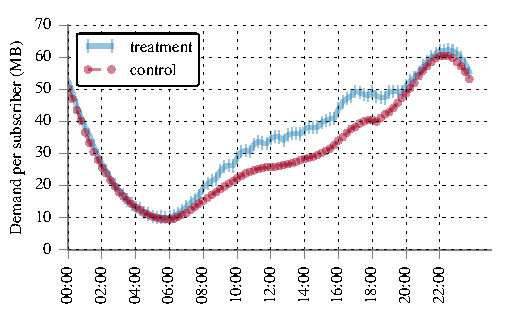
\includegraphics[width=\linewidth]{figures/weekday_demand_mean.pdf}
               \caption{Weekday traffic demand\label{fig:weekday-daily-usage}}
\end{subfigure}
%
\begin{subfigure}[b]{.99\linewidth}
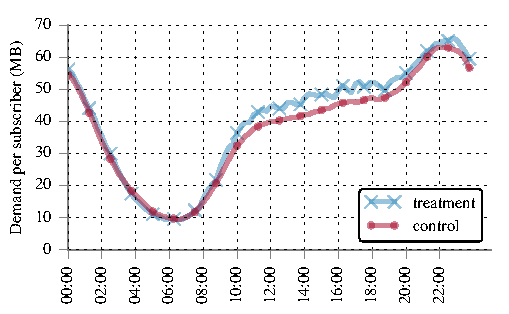
\includegraphics[width=\linewidth]{figures/weekend_demand_mean.pdf}
               \caption{Weekend traffic demand\label{fig:weekend-daily-usage}}
\end{subfigure}
%
\end{minipage}
\caption{Average subscriber demand (bytes every 15-minutes)}
\label{fig:traffic-demand-timeseries}
\end{figure}

Figure \ref{fig:traffic-demand-timeseries} shows the downlink traffic demand (bytes)
of an average subscriber over a 15-minute measurement period in a week.
We observe that subscriber behavior differs
significantly on weekdays and weekends. On weekdays, traffic demand 
increases monotonically from morning until prime-time in the evening. On 
weekends, there is a sharp rise in demand in the early morning period. Then, the
demand plateaus until the next sharp rise during the evening prime-time hours.
Previous reports indicate that the aggregate traffic volume for US fixed access
link providers usually troughs during mid-afternoon hours (between 2:00 PM -- 6:00 PM)
~\cite{sandvine20141h}. We do not observe such a trough in the subscriber 
demand in our dataset.

\begin{figure}[t]
\begin{minipage}{1\linewidth}
\centering
%
\begin{subfigure}[b]{1\linewidth}
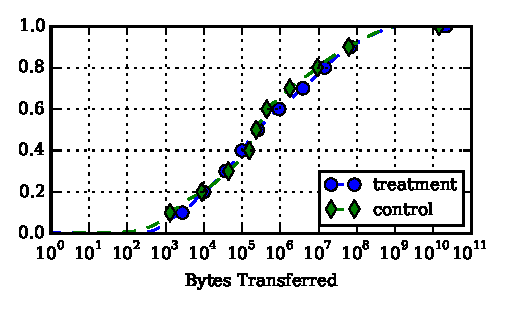
\includegraphics[width=\linewidth]{figures/cdf-all-bytes.pdf}
               \caption{Overall traffic demand for all subscribers at all times\label{fig:CDF-data-rate}}
\end{subfigure}
% maybe should be mean per day?
%
\begin{subfigure}[b]{1\linewidth}
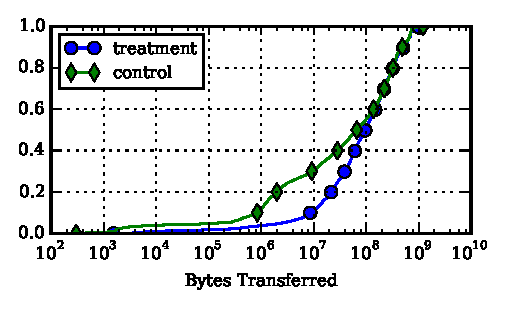
\includegraphics[width=\linewidth]{figures/cdf-per-device-perc95.pdf}
               \caption{Peak (95\%) traffic demand per subscriber\label{fig:CDF-data-rate-perc95}}
\end{subfigure}
%
\end{minipage}
\caption{Traffic demand (bytes every 15-minutes) for \control{} and \treatment{}\label{fig:traffic-demand-cdf}}
\end{figure}

Figure \ref{fig:CDF-data-rate} shows the distribution of the
all bytes transferred in the \treatment{} and \control{} set
over the three months of the dataset. Figure \ref{fig:CDF-data-rate-perc95}
plots the distribution of the peak (95th percentile) demand of the
subscriber over the three months of the dataset. The highest peak
demand achieved by subscribers in the \control{} and \treatment{}
groups were 10 GB in 15-mins. The median peak demand was 80 MB and
100 MB respectively.

We observe that although the overall series are similar, the peak demand of subscribers
is higher in the \treatment{} set. We expected the largest difference
in demands would be in the subscribers who have the heaviest demand already.
But unexpectedly, the lowest demanding 50\% of the subscribers in
\treatment{} have a much higher demand than the lowest demanding 50\% of \control{}.
We confirm that the both groups have similar median demands over each day. However
the daily peak demand is higher for the lowest demanding subscribers in
 \treatment{}, as compared to the lowest demanding subscribers in \control{}.

\begin{figure}[t]
\centering
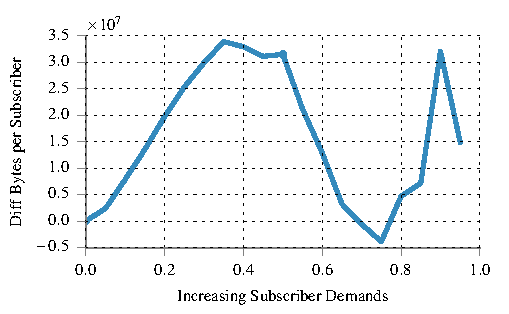
\includegraphics[width=\linewidth]{figures/diff_perc95_bytes_subsc-overall.pdf}
               \caption{Difference between \treatment{} and \control{}
               in peak (95\%) traffic demand\label{fig:diff-perc95}}
\end{figure}

We plot the distribution of the difference in peak subscriber demands for
the lowest to highest demanding subscribers in both groups (Figure~\ref{fig:diff-perc95}).
We see that the peak demand for the lowest demanding 70\% of the households of
the \treatment{} group is higher than the peak demand of the lowest demanding bottom-most
70\% of the \control{} group. These subscribers have a peak demand less than 200 MB.
For 20\% of the subscribers in the \control{} group with peak demands between 10 -- 70 MB,
the equivalent 20\% of the \treatment{} group has peak demands increased by 30 MB.

Under 15\% of subscribers in the \treatment{} group with peak demands more than 200 MB 
peak demands similar, or lower than the equivalent 15\% of subscribers in the \control{}
group, that has a lower capacity. The highest demanding subscribers in the \treatment{}
(beyond 800 MB peak demand) have demands 15 -- 30 MB more than the equivalent 15\% of 
the \control{} group. For the upstream, the \treatment{} group consistently has
a 2 MB higher peak traffic demand every 15 minutes as compared to the \control{} group
(except for the top 10\% users in the \treatment{} set who had a higher peak).

\begin{figure}[t]
\centering
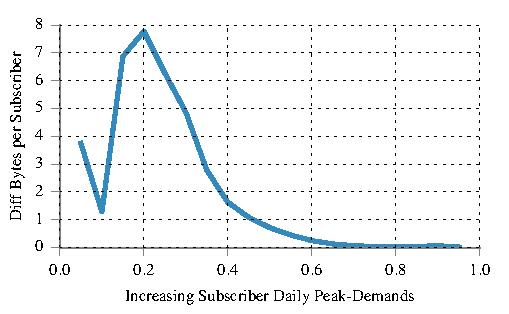
\includegraphics[width=\linewidth]{figures/diff_perc95_bytes_subsc-daily-normalized.pdf}
               \caption{Ratio of the difference between \treatment{} and \control{}
               in the daily peak traffic demand to the daily peak of the \control\label{fig:daily-ratio-perc95}}
\end{figure}

On investigating further, we observed that a similar percentage of 
subscribers with low peak demand in \control{} had a higher peak demand in \treatment{}.
40\% of the subscribers with lowest daily peak demands in the \treatment{} still
had more than double the traffic demand of the equivalent 40\% in the \control{} group.
(see Figure~\ref{fig:daily-ratio-perc95})

the 
There is negligible change in the daily peak 
demand for users who have high demands, and a large increase for users with a low demand.
Furthermore, we observe this affect is also present in the uplink.
There could be many reasons for this increase in demand, such as short
term activities (short videos or web browsing) 
that have a slightly higher traffic demand. Studying the applications 
responsible for such behavioral changes in traffic demand is out of the
scope of this paper and we leave it to future work.

\subsection{User Taxonomy based on Peak Ratio}
\label{subsec:peakratio}
% the ratio of the 90\%-ile to the median throughput per day.

\begin{figure}[ht!]
\begin{minipage}{0.90\linewidth}
\centering
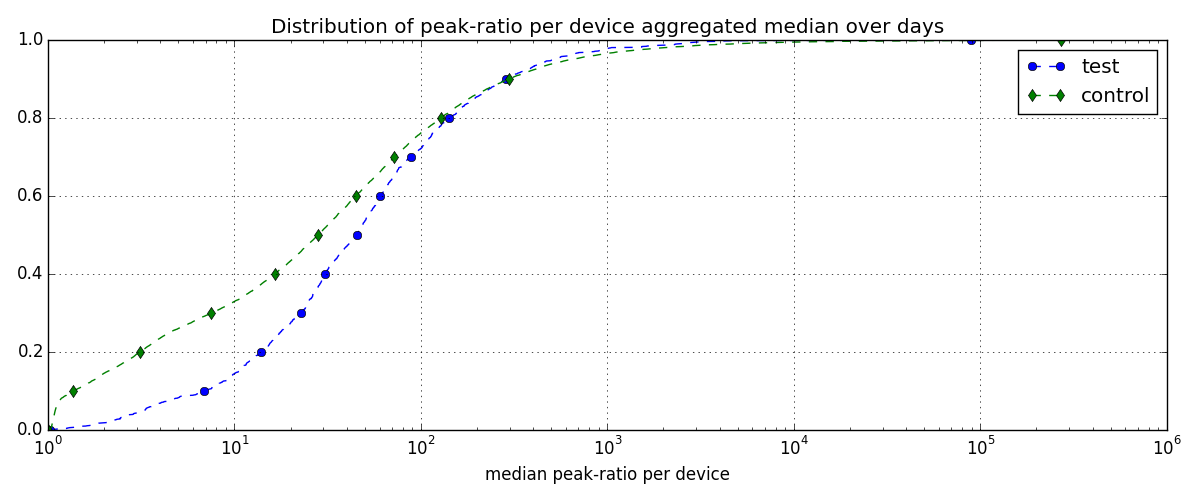
\includegraphics[width=1\linewidth]{figures/peakratio-CDF-devices-MEDIAN.png}
\caption{Median peak ratio per device showing that test set has higher daily ratio (50 times by median). Thus ISPs should condition their networks to 50 times the median usage for each user added in the worst case scenario.}
%http://sites.noise.gatech.edu/~sarthak/files/comcast/plots/full_dw/peakratio-CDF-devices-MEDIAN.png
\label{fig:CDF-peak-ratio-median}
\end{minipage}
\end{figure}

\paragraph{Peak Ratio: }To further characterize and compare the deviation of data rate for the \control and \test set, we examine \emph{peak-ratio} as defined in ~\ref{sec:methodology} 
Figure ~\ref{fig:CDF-peak-ratio-median} shows that the median peak-ratio for each device in the \test set is much larger than that of the \control set.
\todo{replace much larger with the exact number or percentage}.
\sg{Taken together} with our observations of a lower prime-time ratio of the \test set (section~\ref{subsec:primetime}) this implies that there are households in the \test set that achieve a peak-ratio $>$ 1, but not during the prime-time hour. We believe that these households might actually be small businesses or work-at-home users that peak during daytime hours instead of evening hours.

\begin{figure}[ht!]
\begin{minipage}{0.9\linewidth}
\centering
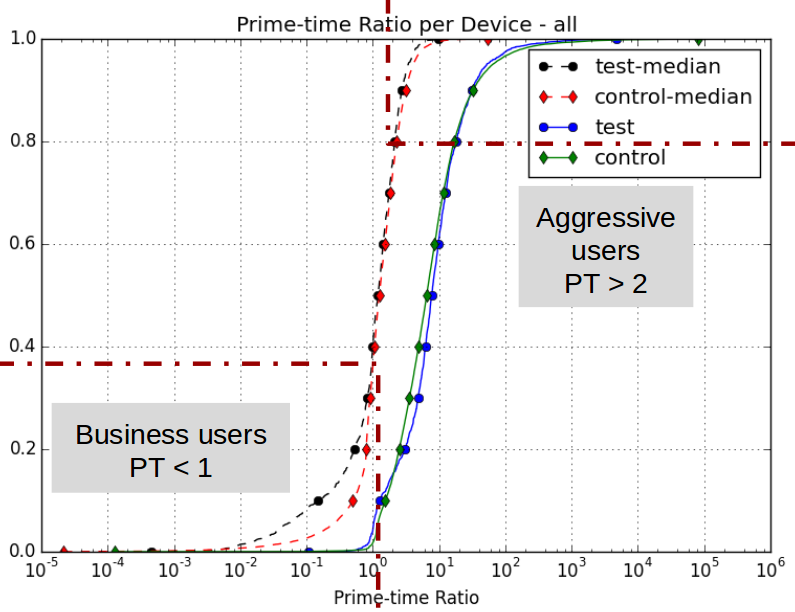
\includegraphics[width=0.9\linewidth]{figures/cdf-prime-time-ratio[replace].png}
\caption{(old) Prime Time ratio + usage can be used to divide users into four sets: aggressive all time + non aggressive all time, aggressive peak time, aggressive non-peak time (business hours). 30\% PT $<$ 1: possibly businesses with normal work-hours . 20\% PT $>$ 2: aggressive prime-time streamers}
%http://riverside.noise.gatech.edu:8083/separated/full/cdf-prime-time-ratio-per-device.png\\
%http://riverside.noise.gatech.edu:8083/plots/full_dw/prime-time-ratio-per-device-cdf-ALL.png
\label{fig:CDF-prime-time-ratio}
\end{minipage}
\end{figure}

The median peak-ratio per device itself shows a large range, from 1 to 10e6 (figure~\ref{fig:CDF-peak-ratio-median}), and the maximum peak-ratio per device was an order higher. Clearly there are some households that have a very even usage throughout the day (low peak ratio), and others that are extremely aggressive only at certain times (high peak ratio). We plot this segregation in figure ~\ref{fig:CDF-prime-time-ratio}.

\todo{EVERYTHING BELOW THIS IS TODO AND TODISCUSS}

\paragraph{User Taxonomy:} The Sandvine reports present a taxonomy of users based on their contribution to real-time entertainment traffic. We incorporate a similar definition based on contribution to data traffic, along with our observations of utilization, to present a taxonomy of the users in our dataset. One category of users is the non-utilizers, i.e., non-aggressive low bandwidth users, that contribute less than SOME THRESHOLD PERCENTILE to the daily data transferred \sg{these the ISP can ignore, also they probably don't need this tier as their utilization from the previous section must be super low}. The second category is of users contributing most aggressively to the data at the ISP \sg{these users will probably gobble up a higher capacity link if given a chance - they're the ones who effect all our graphs.. Need to check this claim}. We further subdivide this high utilizing subcategory based on differing prime-time ratio and peak-ratios follows... \todo{need to think and analyze this further: technical definition to do the analysis}
\begin{itemize}
\item Aggressive All-Time: Users having a low peak-ratio due to a lower variance. Is also expected to have a low prime-time ratio.
\item Aggressive Prime-Time: The usual streamer with a high prime-time ratio and a high peak ratio.
\item Aggressive Non-Prime-Time: Possibly a business user with a low prime-time ratio  but a high peak ratio
\end{itemize}

% other results:
%big difference (2 x median ratio) in per device per day ratios of 90%ile:median.
%weird shape again for values < ratio 100
%big difference in this ratio per day, and it is consistent across all individual sets + months.
%very large for Dec, slightly smaller for Nov
%interestingly, at higher ratios control is slightly > test. This means that certain devices in control set have a huge std (ratio) in a day as compared to test set which has a lower “max” ratio.

\todo{ TO PLOT :}
\begin{itemize}
\itemsep0em
\item peak ratio cdf vs no of devices
\item peak ratio cdf vs time of day where peak occurred
\item no of devices cdf vs time of day where peak occurred
\end{itemize}

Based on differing usage profiles within the same high tier bandwidth, we suggest that the FCC adopt multiple benchmarks based on usage characteristics to better characterize broadband availability, deployment, and adoption in the US. Such multiple benchmarks can be the minimum broadband speed required per user based on the kind of traffic expected during a day. ISPs can also offer these users better plans based on hour-of-the-day or usage caps to encourage more off-peak usage. These users probably don't cause latency spikes in PT.


We recommend multiple standards...

\subsection{Prime-Time Ratio} \label{subsec:primetime}

The daily diurnal nature of Internet traffic demand requires that ISP providers 
design networks capable of handling load at the times when heaviest usage is 
observed. Such heavy demand is usually observed during prime time hours in the 
evening, when many subscribers heavily consume real-time entertainment traffic
(video) (seen as primarily responsible for high usage during these hours). The FCC defines 
Prime-Time as the local time from 7:00 PM to 11:00 PM.
\cite{fcc2014measuring-broadband}. To measure the concentration of network usage
during prime-time, we use Sandvine's definition of the \emph{Prime-Time 
ratio}: the ratio of the average traffic demand during prime-time hours to the average 
traffic demand in non-prime-time hours.\cite{sandvine20141h, sandvine20142h}.

We measure the prime-time ratio of the \control{} and \treatment{} group
for each contiguous four hour period in our datasets to find the evening hours with
the largest prime-time ratio. We observed that in our dataset,
the prime time ratio consistently peaks at 8:00 PM -- 12:00 AM for both
datasets.

%\begin{figure}[t]
%\begin{minipage}{1\linewidth}
%\centering
%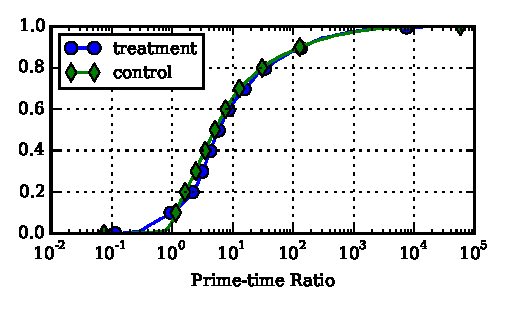
\includegraphics[width=1\linewidth]{figures/prime-time-ratio-per-device-cdf-MEAN.pdf}
%\caption{Prime-Time Ratio\label{fig:cdf-prime-time-ratio}}
%\end{minipage}
%\end{figure}

%\begin{subfigure}[]{.32\linewidth}
%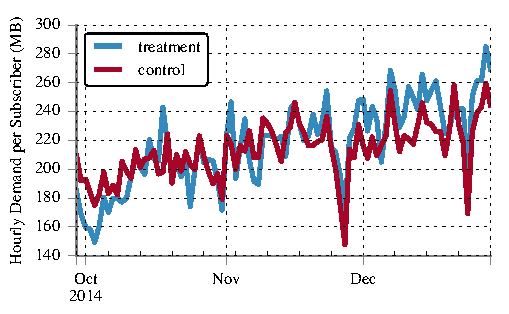
\includegraphics[width=1\linewidth]{figures/primetime_usage_per_day_per_subs.pdf}
%\caption{\label{fig:pt}}
%\end{subfigure}

%\begin{subfigure}[b]{.32\linewidth}
%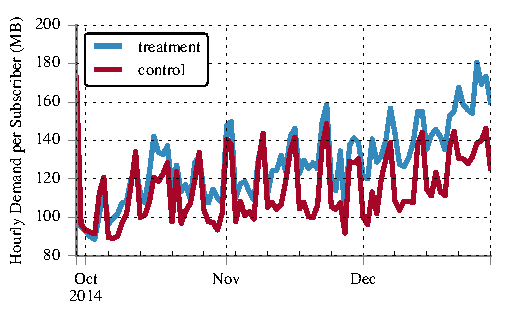
\includegraphics[width=1\linewidth]{figures/nonprimetime_usage_per_day_per_subs.pdf}
%\caption{\label{fig:non-pt}}
%\end{subfigure}


We observed that the hourly downlink traffic per 1000 subscribers between 8:00 PM -- 12:00 AM is 
209.5 GB for \treatment{}, and 205.1 GB for \control{}. However, during an average hour
outside of prime time, the traffic per 1000 subscribers is 122.3 GB for the higher tier
and 108.5 GB for the lower tier. This difference in demand during hours outside of the
daily prime-time is also apparant from the weekly usage patterns in Figure~\ref{fig:traffic-demand-timeseries}.

\begin{table}[t]
\begin{tabular}{| cc | c |c | }\hline
  &                    & Weekday         & Weekends \\\hline
\multirow{2}{*}{\begin{tabular}[c]{@{}l@{}}Hourly Traffic in\\ Prime-Time\end{tabular}}
& treatment          & 233.12          & 246.93   \\
& control            & 225.40          & 238.15   \\\hline
\multirow{2}{*}{\begin{tabular}[c]{@{}l@{}}Hourly Traffic in\\ Non-Prime-Time\end{tabular}}
& treatment & 124.18 & 143.08    \\
& control   & 104.30  & 133.16  \\\hline
\multirow{2}{*}{\begin{tabular}[c]{@{}l@{}}Prime-Time Ratio\end{tabular}}
& treatment & \textbf{1.88} &  1.73 \\
& control  &  \textbf{2.16} &  1.79 \\\hline
\end{tabular}
\caption{Hourly Traffic Demand during in prime-time hours (MB)\label{prime-time-demand}}
\end{table}


We calculate the prime-time ratio per day for the 
datasets groups over weekends and weekdays, as shown in Table \ref{prime-time-demand}.
%in figure~\ref{fig:cdf-prime-time-ratio}. A comparison shows 
On weekends, the prime-time ratios for both groups are
1.73 and 1.79 respectively. On the weekdays, the prime-time ratio for \control{}
is much higher, 2.16, as compared to treatment, 1.88. The demand
during prime-time hours on the weekdays for \treatment{} is within 4\% of
the \control{} traffic, thus there is no substantial
change. In contrast, the demand in non-prime-time hours (outside 8:00 PM -- 12:00 PM)
is much higher in the \treatment{} group, especially on weekdays. 

By definitition, the prime-time ratio is measured using total traffic volume in a day.
For our dataset, the prime-time ratio for the \treatment and \control groups
were 1.70 and 1.93 respectively. However, not all subscribers contribute equally
to the traffic volume. We observed that the median prime-time ratio \emph{per subscriber}
is 3.39 for the \treatment{} group and 2.91 for the \control{} group. This indicates
that demand during prime-time per subscriber has increased, but the total
traffic volume during non-prime-time hours has also increased substantially. For
subscribers that have a larger aggregate demand during non-prime-time hours, the prime
time ratio will be less than one. We found 9\% of the \control{} group and 14\% of 
the treatment group showed this behavior. These subscribers may be small home-run businesses,
users who work at home, or just users who have unexpected usage behaviors. 6\% of the 
subscribers in both groups had a prime-time ratio over 100.

Thus the overall demand of subscribers in the \treatment{} may have decreased by 
total volume of traffic, however, it has increased on a per-subscriber basis.
This result indicates that individual subscribers that do not contribute substantially
to the traffic volume are the ones who have higher usage in prime-time as compared to their
lower tier counterparts.

%Latency and performance 
%are adversely affected during prime-time, causing bottlenecks at home, the last 
%mile, in
%transit, or at the content server. For example, the Sandvine Global
%Internet Phenomena Report \footnote{The Sandvine Reports ~\cite{sandvine20141h,
%sandvine20142h}are released bi-annually and
%contain a detailed analysis of aggregate Internet usage. They are also referred
%to in the FCC reports~\cite{fcc2015progress-report, fcc2014measuring-broadband,
%fcc2014progress-report}} showed that devices in the same household selected  
%Netflix's own CDN (OpenConnect) during off-peak hours, and third party CDNs 
%(with differing
%performance) during prime-time. This may happen because Netflix OpenConnect is
%over-utilized during prime time~\cite{sandvine20141h}.

\subsection{Aggressive Subscribers}\label{subsec:prevalence}

\begin{figure}[ht]
\begin{minipage}{\linewidth}
\centering
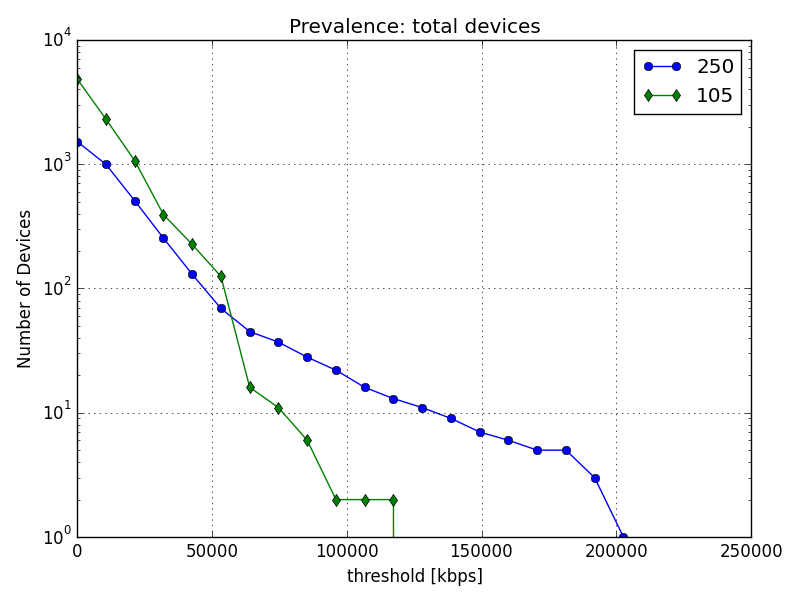
\includegraphics[width=\linewidth]{figures/prevalence.png}
\caption{User prevalence as threshold increases.}
\label{fig:prevalence}
\end{minipage}
\end{figure}

Outliers. Prevalence.
While the general behavior did not change, still 11 users maxed out traffic.
For example (explain the fig)

\balance\section{Conclusion}\label{sec:conclusion}\label{lastpage}

\section*{Acknowledgments}

This research was supported by the Comcast Tech Research Fund and by NSF
Awards CNS-1539902 and CNS-1540066. We thank Jason Livingood and James
Moon from Comcast for helpful discussions and access to the data that we
used for this study.


\end{sloppypar}

%\vspace{-0.1in}
%\section*{Acknowledgments}
% Comments for people we need to acknowledge in the final version.
%We would like to thank the anonymous XXX reviewers and our shepherd, ...

%\pagebreak

\small
%\setlength{\bibsep}{0pt}
\setlength{\parskip}{-1pt}
\setlength{\itemsep}{-1pt}
% \footnotesize % SPACE
\balance\bibliography{paper}
\bibliographystyle{abbrv}
%\bibliographystyle{abbrvnat_noaddr} % SPACE
%\theendnotes % ENDNOTES
%}

\end{document}

%%%%%%%%%%%%%%%%%%%%  END OF DOCUMENT  %%%%%%%%%%%%%%%%%%%%
